\section{离散分布}
\label{sec:cdist-discrete}

离散模型的取值可以一个一个列出来，概率由质量函数给出。建立这样的模型有固定的步骤：先说清基本试验是什么，各次试验之间有没有牵连，随机变量记录的又是什么；再用计数和第~\ref{chap:classical-probability}章的乘法规则推出质量函数，核对它非负、总和为一；最后计算期望和方差。

参数的名字相近，并不说明试验机制相同。二项分布和几何分布都有一个“成功概率$p$”，但前者固定试验次数、数成功的个数，后者固定只等一次成功、数试验的次数。二项分布和超几何分布都有一个“抽取个数$n$”，但前者各次互不影响，后者每抽走一个都会改变剩下的构成。下面五个模型都用开头那条生产线演示，便于比较。

\subsection{Bernoulli分布}
\label{sec:cdist-bernoulli}

最简单的随机记录只有两种结果：零件是次品或不是，硬币是正面或反面。把关心的那种结果叫作“成功”，记为$1$，另一种记为$0$，就得到只取两个值的随机变量。它的分布只需要一个数来描述。

\begin{definition}[Bernoulli分布]
\label{def:cdist-bernoulli}
设$0\leq p\leq1$。若随机变量$X$只取$0,1$两个值，且
\begin{equation}
  \mathbb{P}(X=1)=p,\qquad \mathbb{P}(X=0)=1-p,
  \label{eq:cdist-bernoulli-pmf}
\end{equation}
则称$X$服从参数为$p$的\term{Bernoulli分布}（Bernoulli distribution），记作$X\sim\operatorname{Bern}(p)$，$p$称为成功概率。
\end{definition}

两个概率也可以合写成一个质量函数$p_X(x)=p^{x}(1-p)^{1-x}$，$x\in\{0,1\}$。这里约定$0^{0}=1$，这样$p=0$或$p=1$时公式仍然成立。

期望按概率加权平均计算：
\[
  \mathbb{E}[X]=0\cdot(1-p)+1\cdot p=p .
\]
$X$只取$0$和$1$，所以$X^{2}=X$，于是$\mathbb{E}[X^{2}]=p$。代入第~\ref{chap:random-variable-moments}章的方差展开式，即二阶矩减去期望的平方，得到
\begin{equation}
  \mathbb{E}[X]=p,\qquad \operatorname{Var}(X)=p(1-p).
  \label{eq:cdist-bernoulli-moments}
\end{equation}

把概率看成质量，就能看出这两个数的含义。点$0$上放质量$1-p$，点$1$上放质量$p$，重心落在$p$处，这就是期望；生产线的例子中$p=0.2$，期望$0.2$并不是$X$能取到的值。方差是质量相对重心的转动惯量，两端质量相等时最大，在$p=1/2$处达到$1/4$；例中方差为$0.16$。图~\ref{fig:cdist-bernoulli-variance}画出了这两点。

\begin{BookInlineFigure}
  \centering
  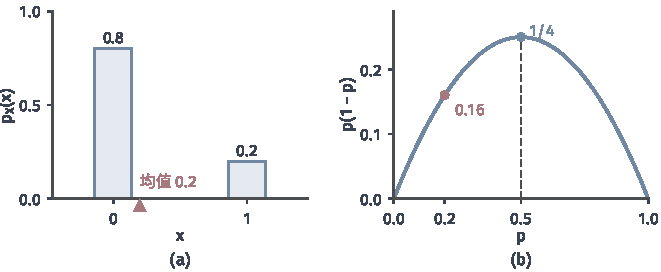
\includegraphics[width=112mm]{figures/07-probability/01-elementary-probability/matplotlib/cdist-bernoulli-variance/figure.pdf}
  \caption{Bernoulli分布。(a)$p=0.2$的质量表，红色三角是期望$0.2$，也就是两根柱子的重心。(b)方差$p(1-p)$随$p$的变化，蓝点为最大值$1/4$（$p=1/2$），红点为例中的$0.16$。}
  \label{fig:cdist-bernoulli-variance}
\end{BookInlineFigure}

端点$p=0$和$p=1$也算Bernoulli分布，但这时$X$以概率一取固定值，方差为零，与第~\ref{chap:random-variable-moments}章“方差为零即以概率一取常数”的结论一致。后面的模型在参数取到端点时也会出现这种退化，届时都要单独核对。

\paragraph{指示变量}
任何事件都可以用一个Bernoulli变量来记录。对事件$A$，令
\begin{equation}
  \mathbf{1}_{A}(\omega)=
  \begin{cases}
    1, & \omega\in A,\\
    0, & \omega\notin A,
  \end{cases}
  \label{eq:cdist-indicator}
\end{equation}
称为$A$的\term{指示变量}（indicator variable）。它在$A$发生时取$1$，否则取$0$，所以$\mathbf{1}_{A}\sim\operatorname{Bern}(\mathbb{P}(A))$，并且
\begin{equation}
  \mathbb{E}[\mathbf{1}_{A}]=\mathbb{P}(A).
  \label{eq:cdist-indicator-mean}
\end{equation}

图~\ref{fig:cdist-indicator}以掷两枚骰子为例。样本空间有$36$个等可能的点，事件$A$为“点数之和不小于$10$”，含$6$个点。指示变量把这$6$个点送到$1$，其余$30$个点送到$0$，得到的质量表是$5/6$与$1/6$，期望正是$\mathbb{P}(A)=1/6$。

\begin{BookInlineFigure}
  \centering
  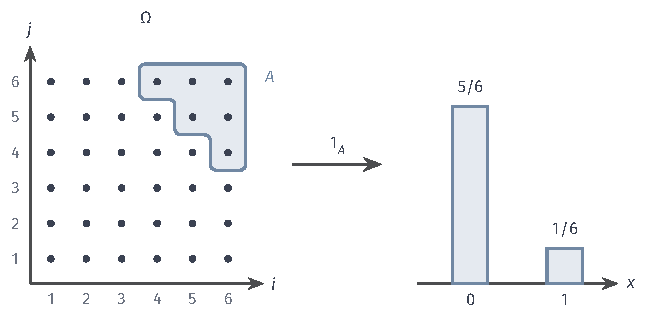
\includegraphics[width=109mm]{figures/07-probability/01-elementary-probability/tikz/cdist-indicator/figure.pdf}
  \caption{指示变量是样本空间上的函数。左：两枚骰子的$36$个样本点，浅蓝区域是事件$A=\{i+j\geq10\}$。右：$\mathbf{1}_{A}$的质量表，$A$中的$6$个点贡献点$1$上的质量$1/6$。}
  \label{fig:cdist-indicator}
\end{BookInlineFigure}

指示变量还有两条代数性质，下面两小节要反复使用。第一条是$\mathbf{1}_{A}^{2}=\mathbf{1}_{A}$，因为$0^{2}=0$、$1^{2}=1$。第二条是乘积等于交事件的指示变量：
\begin{equation}
  \mathbf{1}_{A}\mathbf{1}_{B}=\mathbf{1}_{A\cap B},
  \label{eq:cdist-indicator-product}
\end{equation}
因为两边都在$A$与$B$同时发生时取$1$，否则取$0$。

有了这两条，“$n$个事件中发生了几个”就能写成$\mathbf{1}_{A_1}+\dots+\mathbf{1}_{A_n}$。由期望的线性性和式~\eqref{eq:cdist-indicator-mean}，它的期望等于$\mathbb{P}(A_1)+\dots+\mathbb{P}(A_n)$，这一步对事件之间的任何牵连都成立。计数问题因此可以拆成单个事件的概率来算。

\subsection{二项分布}
\label{sec:cdist-binomial}

连续检查$10$个零件，次品数$X$可能取$0,1,\dots,10$中的任何一个。要写出$\mathbb{P}(X=k)$，先把假设说清楚：每个零件是次品的概率都是$0.2$，而且各零件是否为次品互不影响。

一般地，进行$n$次试验，记$A_i$为“第$i$次成功”，并假设三条：试验次数$n$事先固定；每次成功的概率都是$p$；事件$A_1,\dots,A_n$相互独立。成功的总次数是$n$个指示变量之和，
\[
  X=\mathbf{1}_{A_1}+\mathbf{1}_{A_2}+\dots+\mathbf{1}_{A_n}.
\]

\paragraph{质量函数}
$X=k$意味着恰好有$k$个$A_i$发生。先固定一组成功的位置$S\subseteq\{1,\dots,n\}$，$\lvert S\rvert=k$，考虑事件“$i\in S$时$A_i$发生，$i\notin S$时$A_i$不发生”。相互独立的事件把其中一部分换成补事件后仍然相互独立（第~\ref{chap:classical-probability}章），所以这个事件的概率是$k$个$p$与$n-k$个$1-p$之积：
\[
  p^{k}(1-p)^{n-k}.
\]
这个值只依赖于成功的个数，与成功出现在哪些位置无关。

从$n$个位置中选出$k$个作为成功位置，共有$\binom{n}{k}$种选法，可参考\BookChapterRef{chap:counting}{卷一第2章“计数”}。不同的$S$对应的事件互不相容，把它们的概率加起来，就得到$X$的质量函数。

\begin{definition}[二项分布]
\label{def:cdist-binomial}
设$n$为正整数，$0\leq p\leq1$。若随机变量$X$的质量函数为
\begin{equation}
  \mathbb{P}(X=k)=\binom{n}{k}p^{k}(1-p)^{n-k},\qquad k=0,1,\dots,n,
  \label{eq:cdist-binomial-pmf}
\end{equation}
则称$X$服从参数为$n,p$的\term{二项分布}（binomial distribution），记作$X\sim\operatorname{Bin}(n,p)$。
\end{definition}

由二项式定理，质量函数的总和是$(p+(1-p))^{n}=1$，名字也由此而来。$n=1$时它就是$\operatorname{Bern}(p)$。

图~\ref{fig:cdist-binomial-sequences}把$n=3$、$p=0.2$的八种结果按成功次数分成四组。每一条结果的概率只看其中有几个成功，同组各条相同；组内条数是$\binom{3}{k}$，乘起来就是$\mathbb{P}(X=k)$。

\begin{BookInlineFigure}
  \centering
  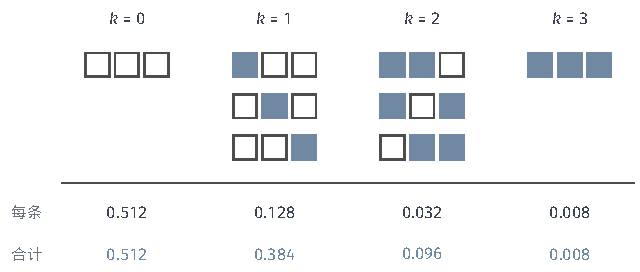
\includegraphics[width=108mm]{figures/07-probability/01-elementary-probability/tikz/cdist-binomial-sequences/figure.pdf}
  \caption{$n=3$次独立试验、$p=0.2$时的八种结果，蓝色方格表示成功。按成功次数$k$分组：每条结果的概率为$p^{k}(1-p)^{3-k}$，组内共$\binom{3}{k}$条，合计即二项概率，四个合计之和为$1$。}
  \label{fig:cdist-binomial-sequences}
\end{BookInlineFigure}

回到$n=10$、$p=0.2$的检查。由式~\eqref{eq:cdist-binomial-pmf}，没有次品和恰有两个次品的概率分别是
\[
  \mathbb{P}(X=0)=0.8^{10}\approx0.1074,\qquad
  \mathbb{P}(X=2)=45\times0.2^{2}\times0.8^{8}\approx0.3020 .
\]
次品不少于$4$个的概率为$1-\mathbb{P}(X\leq3)\approx0.1209$。

\paragraph{形状}
设$0<p<1$，质量函数先升后降。相邻两项之比为
\[
  \frac{\mathbb{P}(X=k+1)}{\mathbb{P}(X=k)}=\frac{(n-k)p}{(k+1)(1-p)},
\]
它大于$1$当且仅当$(n-k)p>(k+1)(1-p)$，整理后即$k<(n+1)p-1$。所以概率在$k$小于$(n+1)p-1$时上升，之后下降，最大值落在$\lfloor(n+1)p\rfloor$处；$(n+1)p$恰为整数时，它和前一个整数并列最大。例中$(n+1)p=2.2$，最可能的次品数是$2$。

把成功与失败对调，$k$次成功就是$n-k$次失败，所以$\operatorname{Bin}(n,1-p)$的质量函数是$\operatorname{Bin}(n,p)$的左右翻转。图~\ref{fig:cdist-binomial-pmf}(b)中$p=0.8$的柱子正是图~\ref{fig:cdist-binomial-pmf}(a)的镜像，$p=0.5$时左右对称。

\begin{BookInlineFigure}
  \centering
  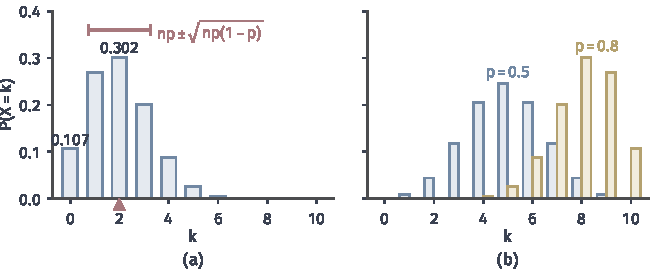
\includegraphics[width=112mm]{figures/07-probability/01-elementary-probability/matplotlib/cdist-binomial-pmf/figure.pdf}
  \caption{二项分布的质量函数，$n=10$。(a)$p=0.2$，红色三角为期望$2$，红色横线标出期望左右各一个标准差$\sqrt{1.6}\approx1.26$的范围。(b)$p=0.5$（蓝）和$p=0.8$（黄），后者是(a)的左右翻转。}
  \label{fig:cdist-binomial-pmf}
\end{BookInlineFigure}

\paragraph{期望与方差}
期望直接由指示变量之和得到。由线性性和式~\eqref{eq:cdist-indicator-mean}，
\[
  \mathbb{E}[X]=\sum_{i=1}^{n}\mathbb{P}(A_i)=np .
\]
这一步没有用到独立性。

方差要先算$\mathbb{E}[X^{2}]$。把平方展开成双重和，并把$i=j$与$i\neq j$的项分开：
\[
  X^{2}=\sum_{i=1}^{n}\sum_{j=1}^{n}\mathbf{1}_{A_i}\mathbf{1}_{A_j}
  =\sum_{i=1}^{n}\mathbf{1}_{A_i}+\sum_{i\neq j}\mathbf{1}_{A_i\cap A_j},
\]
这里用了$\mathbf{1}_{A_i}^{2}=\mathbf{1}_{A_i}$和式~\eqref{eq:cdist-indicator-product}。第二个和共有$n(n-1)$个有序对$(i,j)$。

对两边取期望。由独立性，$i\neq j$时$\mathbb{P}(A_i\cap A_j)=p^{2}$，于是
\[
  \mathbb{E}[X^{2}]=np+n(n-1)p^{2}.
\]
再减去期望的平方，
\[
  \operatorname{Var}(X)=np+n(n-1)p^{2}-n^{2}p^{2}=np-np^{2}.
\]
合起来就是
\begin{equation}
  \mathbb{E}[X]=np,\qquad \operatorname{Var}(X)=np(1-p).
  \label{eq:cdist-binomial-moments}
\end{equation}
例中期望为$2$，方差为$1.6$，标准差约$1.26$。

\paragraph{三个量的区分}
二项模型里有三个量，含义各不相同。试验次数$n$是事先设计好的，成功概率$p$是模型的参数，$X$则是试验做完才看到的计数。看到$X=3$并不等于知道$p=0.3$，由观察到的计数反推$p$属于统计推断，可参考\BookChapterRef{chap:parametric-statistical-inference}{卷八第1章“参数化统计推断”}。

\paragraph{去掉条件会怎样}
三条假设少了任何一条，式~\eqref{eq:cdist-binomial-pmf}都不再成立。先看成功概率不相同的情形：两次试验相互独立，第一次必然失败，第二次必然成功。成功次数恒为$1$，方差为零；平均成功概率同样是$1/2$的$\operatorname{Bin}(2,1/2)$却有方差$1/2$。

再看独立性。假设$10$个零件出自同一副模具，要么全是次品，要么全是合格品，前者的概率为$0.2$。此时每个零件仍以$0.2$的概率是次品，次品数只取$0$和$10$，期望仍是$2$。可方差变成了
\[
  \mathbb{E}[X^{2}]-(\mathbb{E}[X])^{2}=0.2\times100-4=16,
\]
是二项模型的十倍。期望的计算不需要独立性，方差却完全取决于事件之间的牵连。

\subsection{超几何分布}
\label{sec:cdist-hypergeometric}

一箱$N=20$个零件中恰有$K=4$个次品，从中不放回地取出$n=10$个。这时次品数$X$不再服从二项分布：每取走一个次品，剩下的次品比例就变小，各次抽取互相牵连。我们回到古典模型，直接计数。

\paragraph{质量函数}
把一次抽样记作从$N$个零件中选出的一个$n$元子集，共有$\binom{N}{n}$个，按假设它们等可能。$X=k$的子集要从$K$个次品中选$k$个、从$N-K$个合格品中选$n-k$个，共有$\binom{K}{k}\binom{N-K}{n-k}$个。$k$还要同时满足$k\leq K$、$k\leq n$和$n-k\leq N-K$，这给出了取值范围。

\begin{definition}[超几何分布]
\label{def:cdist-hypergeometric}
设$N$为正整数，整数$K,n$满足$0\leq K\leq N$，$0\leq n\leq N$。若随机变量$X$的质量函数为
\begin{equation}
  \mathbb{P}(X=k)=\frac{\binom{K}{k}\binom{N-K}{n-k}}{\binom{N}{n}},\qquad
  \max(0,n-N+K)\leq k\leq\min(n,K),
  \label{eq:cdist-hypergeometric-pmf}
\end{equation}
则称$X$服从\term{超几何分布}（hypergeometric distribution），记作$X\sim\operatorname{Hyp}(N,K,n)$。
\end{definition}

各项之和为一，是因为每个$n$元子集恰好含有某个数目的次品，把子集按次品数分组计数，各组个数之和就是$\binom{N}{n}$。

例中$\binom{20}{10}=184756$。按次品数$0,1,2,3,4$分组，子集个数分别是$8008$、$45760$、$77220$、$45760$、$8008$，对应的概率为
\[
  0.0433,\quad 0.2477,\quad 0.4180,\quad 0.2477,\quad 0.0433 .
\]
次品数为$4$（全部次品都被抽中）的概率是$0.0433$，而二项模型中“不少于$4$个”的概率是$0.1209$。

\paragraph{期望}
直接从式~\eqref{eq:cdist-hypergeometric-pmf}求和比较繁琐，改用指示变量。把$n$个零件按抽出的先后排成序列，所有$N(N-1)\cdots(N-n+1)$个有序序列等可能，因为每个子集恰对应$n!$个排列。记$B_i$为“第$i$个抽出的是次品”，则$X=\mathbf{1}_{B_1}+\dots+\mathbf{1}_{B_n}$。

数一数第$i$个位置是次品的序列：这个位置有$K$种选法，其余$n-1$个位置依次有$N-1,N-2,\dots,N-n+1$种选法。与全部序列数相比，得到
\[
  \mathbb{P}(B_i)=\frac{K\,(N-1)(N-2)\cdots(N-n+1)}{N(N-1)\cdots(N-n+1)}=\frac{K}{N}.
\]
这与位置$i$无关：在一无所知的时候，第$i$个抽出的零件可以是$N$个中的任何一个，机会均等。由线性性，
\begin{equation}
  \mathbb{E}[X]=n\frac{K}{N}.
  \label{eq:cdist-hypergeometric-mean}
\end{equation}

\paragraph{方差与有限总体修正}
仿照二项分布，需要两个位置同时为次品的概率。设$N>1$，$i\neq j$，同样数序列：
\[
  \mathbb{P}(B_i\cap B_j)=\frac{K(K-1)}{N(N-1)} .
\]
代入$X^{2}$的双重和展开，得到
\[
  \mathbb{E}[X^{2}]=n\frac{K}{N}+n(n-1)\frac{K(K-1)}{N(N-1)} .
\]

记$r=K/N$，则$(K-1)/(N-1)=(rN-1)/(N-1)$。减去$(nr)^{2}$并提出公因子$nr$：
\[
  \operatorname{Var}(X)=nr\Bigl[1+(n-1)\frac{rN-1}{N-1}-nr\Bigr].
\]
方括号通分后，分子为
\[
  (N-1)+(n-1)(rN-1)-nr(N-1)=N-n-rN+rn=(N-n)(1-r).
\]
于是得到
\begin{equation}
  \operatorname{Var}(X)=n\frac{K}{N}\Bigl(1-\frac{K}{N}\Bigr)\frac{N-n}{N-1},\qquad N>1 .
  \label{eq:cdist-hypergeometric-var}
\end{equation}

与有放回抽样比较最能看出这个公式的含义。有放回时各次抽取独立，次品数服从$\operatorname{Bin}(n,K/N)$，期望同为$nK/N$，方差为$n(K/N)(1-K/N)$。不放回抽样的方差多了一个因子$(N-n)/(N-1)$，称为\term{有限总体修正}（finite population correction）。

因子小于一的原因在于两次抽取的负牵连。$K<N$时$(K-1)/(N-1)<K/N$，所以$\mathbb{P}(B_i\cap B_j)<\mathbb{P}(B_i)\mathbb{P}(B_j)$：前一个抽到次品，后一个抽到次品的机会就变小，次品数因此不容易偏离均值太远。例中方差为$1.6\times10/19\approx0.842$，只有二项模型的一半略多，见图~\ref{fig:cdist-hypergeom-binomial}(a)。

\begin{BookInlineFigure}
  \centering
  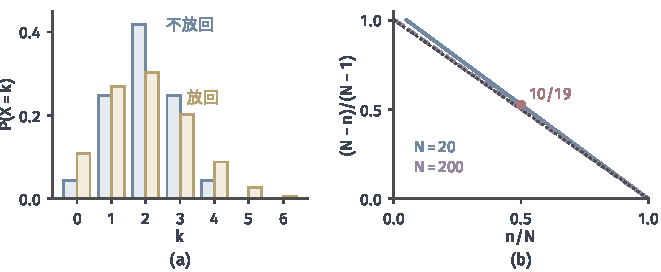
\includegraphics[width=112mm]{figures/07-probability/01-elementary-probability/matplotlib/cdist-hypergeom-binomial/figure.pdf}
  \caption{不放回与放回抽样。(a)$N=20$、$K=4$、$n=10$时次品数的分布：蓝色为$\operatorname{Hyp}(20,4,10)$，黄色为放回抽样的$\operatorname{Bin}(10,0.2)$，两者期望都是$2$。(b)有限总体修正$(N-n)/(N-1)$随抽样比例$n/N$的变化，$N=20$（蓝）与$N=200$（紫，虚线），点线为$1-n/N$；红点是例中的$10/19$。}
  \label{fig:cdist-hypergeom-binomial}
\end{BookInlineFigure}

\paragraph{边界情形}
修正因子在两端退化。$n=N$时因子为零，整箱都被取出，$X$恒等于$K$。$n=1$时因子为一，只抽一个，$X\sim\operatorname{Bern}(K/N)$。$K=0$或$K=N$时箱中只有一类零件，$X$也是常数，式~\eqref{eq:cdist-hypergeometric-var}同样给出零。$N=1$时公式的分母为零，此时$n\in\{0,1\}$，$X$只能是常数或一个Bernoulli变量，直接计算即可。

\paragraph{何时可以用二项分布近似}
总体很大而抽样比例很小时，取走几个零件几乎不改变剩下的构成，不放回与放回就相差无几。设$K/N\to r$且$N\to\infty$，$n$和$k$固定。把式~\eqref{eq:cdist-hypergeometric-pmf}的组合数展开成乘积并重新分组：
\[
  \mathbb{P}(X=k)=\binom{n}{k}
  \prod_{j=0}^{k-1}\frac{K-j}{N-j}\prod_{j=0}^{n-k-1}\frac{N-K-j}{N-k-j}.
\]
第一个乘积的每个因子趋于$r$，第二个乘积的每个因子趋于$1-r$，所以概率趋于$\binom{n}{k}r^{k}(1-r)^{n-k}$。

修正因子告诉我们误差的量级：它约等于$1-n/N$。例如$N=2000$、$K=400$、$n=10$时因子为$1990/1999\approx0.9955$，两个模型的方差只差约$0.5\%$；图~\ref{fig:cdist-hypergeom-binomial}(b)中$N=200$的曲线也几乎贴着$1-n/N$。反过来，抽样比例达到一半时，忽略修正会把方差高估将近一倍。

\subsection{几何分布}
\label{sec:cdist-geometric}

现在换一种记录方式：一个一个检查零件，直到遇到第一个次品为止，记$T$为检查的个数（包括这个次品）。二项分布固定次数、数成功；这里只等一次成功，次数本身成了随机的。

设各次试验相互独立，成功概率都是$p$，并要求$0<p\leq1$。$T=k$意味着前$k-1$次都失败、第$k$次成功，由独立性，这个事件的概率是$(1-p)^{k-1}p$。$p=0$时永远等不到成功，$T$没有定义，所以排除在外；$p=1$时$T$恒为$1$。

\begin{definition}[几何分布]
\label{def:cdist-geometric}
设$0<p\leq1$。若随机变量$T$的质量函数为
\begin{equation}
  \mathbb{P}(T=k)=(1-p)^{k-1}p,\qquad k=1,2,\dots,
  \label{eq:cdist-geometric-pmf}
\end{equation}
则称$T$服从参数为$p$的\term{几何分布}（geometric distribution），记作$T\sim\operatorname{Geom}(p)$。
\end{definition}

这是第一个取值无穷多的模型，总和为一要靠级数。记$q=1-p$，由几何级数$\sum_{k\geq1}q^{k-1}=1/(1-q)$，质量函数之和为$p/(1-q)=1$。

“首次成功晚于第$k$次”等价于“前$k$次全部失败”，所以尾概率有简单的形式：
\begin{equation}
  \mathbb{P}(T>k)=(1-p)^{k},\qquad k=0,1,2,\dots .
  \label{eq:cdist-geometric-tail}
\end{equation}
生产线的例子中$p=0.2$，查了$5$个还没遇到次品的概率是$0.8^{5}\approx0.328$，查了$10$个仍没有的概率约为$0.107$。

\paragraph{期望}
对取正整数值的变量，期望可以写成尾概率之和。把$k$写成$k$个$1$相加，再交换求和次序：
\[
  \mathbb{E}[T]=\sum_{k\geq1}k\,\mathbb{P}(T=k)=\sum_{k\geq1}\sum_{j=1}^{k}\mathbb{P}(T=k)
  =\sum_{j\geq1}\sum_{k\geq j}\mathbb{P}(T=k).
\]
所有项都非负，非负项的二重级数按任何次序求和结果相同，所以交换是允许的。内层和就是$\mathbb{P}(T\geq j)=q^{j-1}$，于是
\[
  \mathbb{E}[T]=\sum_{j\geq1}q^{j-1}=\frac{1}{1-q}=\frac1p .
\]

\paragraph{方差}
二阶矩用同样的办法。把$k^{2}$写成前$k$个奇数之和，$k^{2}=\sum_{j=1}^{k}(2j-1)$，交换次序后
\[
  \mathbb{E}[T^{2}]=\sum_{j\geq1}(2j-1)\,\mathbb{P}(T\geq j)=2\sum_{j\geq1}jq^{j-1}-\sum_{j\geq1}q^{j-1}.
\]
第一个和可以借助刚才的结果，把它看成$\mathbb{E}[T]$除以$p$：
\[
  \sum_{j\geq1}jq^{j-1}=\frac1p\sum_{j\geq1}j\,pq^{j-1}=\frac{\mathbb{E}[T]}{p}=\frac{1}{p^{2}}.
\]
于是
\[
  \mathbb{E}[T^{2}]=\frac{2}{p^{2}}-\frac1p .
\]
减去$(\mathbb{E}[T])^{2}=1/p^{2}$，得到
\begin{equation}
  \mathbb{E}[T]=\frac1p,\qquad \operatorname{Var}(T)=\frac{1-p}{p^{2}} .
  \label{eq:cdist-geometric-moments}
\end{equation}
例中平均要查$5$个，方差为$20$，标准差约$4.47$，与均值相当。等待次数的波动很大：前面算过，查到均值的两倍即$10$个仍未遇到次品，概率还超过十分之一。

\paragraph{无记忆性}
已经连续查了$m$个合格品，还要再查多少个？用条件概率计算。因为$\{T>m+k\}\subseteq\{T>m\}$，交事件就是$\{T>m+k\}$，由式~\eqref{eq:cdist-geometric-tail}，
\[
  \mathbb{P}(T>m+k\mid T>m)=\frac{\mathbb{P}(T>m+k)}{\mathbb{P}(T>m)}=\frac{q^{m+k}}{q^{m}}=q^{k}.
\]
它恰好等于$\mathbb{P}(T>k)$。已经失败了多少次，不影响还要等待的次数的分布，这一性质称为\term{无记忆性}（memorylessness）。

图~\ref{fig:cdist-geometric-memoryless}(b)中，从第$5$次之后重新开始数的条件尾概率（绿点）与原来的尾概率（蓝线）完全重合。“已经连着五个合格，下一个该是次品了”的想法，在独立试验中不成立。反过来，若次品成批出现，前面的结果就携带了信息，无记忆性随独立性一起失去。

\begin{BookInlineFigure}
  \centering
  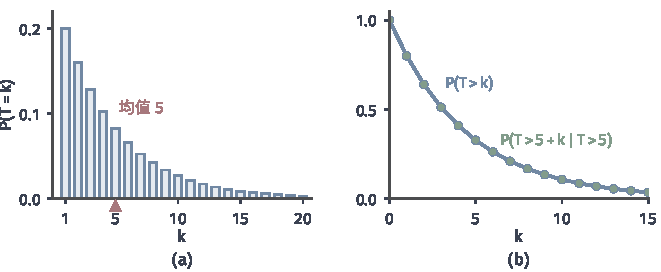
\includegraphics[width=112mm]{figures/07-probability/01-elementary-probability/matplotlib/cdist-geometric-memoryless/figure.pdf}
  \caption{$\operatorname{Geom}(0.2)$。(a)质量函数，红色三角为期望$5$。(b)尾概率$\mathbb{P}(T>k)=0.8^{k}$（蓝）与已知$T>5$后剩余等待的条件尾概率$\mathbb{P}(T>5+k\mid T>5)$（绿点），两者处处相等。}
  \label{fig:cdist-geometric-memoryless}
\end{BookInlineFigure}

无记忆性不只是几何分布的一个性质，它把几何分布完全刻画了出来。

\begin{theorem}[几何分布的无记忆刻画]
\label{thm:cdist-geometric-memoryless}
设$T$取正整数值，且对每个$k\geq0$有$\mathbb{P}(T>k)>0$。若对所有整数$m,k\geq0$都有
\begin{equation}
  \mathbb{P}(T>m+k\mid T>m)=\mathbb{P}(T>k),
  \label{eq:cdist-memoryless-discrete}
\end{equation}
则存在$0<p<1$使$T\sim\operatorname{Geom}(p)$。
\end{theorem}

\begin{proof}
记$G(k)=\mathbb{P}(T>k)$。$T$取正整数值，所以$G(0)=1$。式~\eqref{eq:cdist-memoryless-discrete}左边等于$G(m+k)/G(m)$，于是对所有$m,k\geq0$，
\[
  G(m+k)=G(m)G(k).
\]
取$m=k-1$并对$k$归纳，得到$G(k)=G(1)^{k}$。

记$q=G(1)$，按假设$q>0$。若$q=1$，则$G(k)=1$对所有$k$成立，即$T$大于每一个整数，这与$T$取正整数值矛盾。所以$0<q<1$。令$p=1-q$，则
\[
  \mathbb{P}(T=k)=G(k-1)-G(k)=q^{k-1}-q^{k}=q^{k-1}p,
\]
这正是式~\eqref{eq:cdist-geometric-pmf}。
\end{proof}

\paragraph{另一种计数约定}
也有人记录首次成功之前的失败次数$N=T-1$。它取值于$\{0,1,2,\dots\}$，质量函数为$(1-p)^{k}p$。平移不改变方差，所以
\[
  \mathbb{E}[N]=\frac{1-p}{p},\qquad \operatorname{Var}(N)=\frac{1-p}{p^{2}},
\]
期望比$\mathbb{E}[T]$少$1$。查阅公式时要先确认采用的是哪一种约定，本卷的$\operatorname{Geom}(p)$一律指包含成功那一次的$T$。

\subsection{Poisson分布}
\label{sec:cdist-poisson}

一块钢板表面的划痕数、一小时内到达的故障报警数，都是在固定的范围内计数。这类计数没有事先给定的试验次数，原则上可以取任何非负整数。它们的共同点是：可能发生的机会很多，每个机会发生的概率很小，而且彼此互不影响。

\paragraph{从二项分布出发}
把钢板等分成$n$个小格，假设每格至多有一道划痕，有划痕的概率为$\lambda/n$，各格互不影响。划痕总数服从$\operatorname{Bin}(n,\lambda/n)$，期望固定为$\lambda$。格子分得越细，越接近“任意位置都可能出现划痕”的情形，于是要看$n\to\infty$时质量函数的极限。

\begin{theorem}[二项分布的Poisson极限]
\label{thm:cdist-binomial-poisson}
设$\lambda>0$，$n>\lambda$，$p_n=\lambda/n$。对每个固定的非负整数$k$，
\begin{equation}
  \lim_{n\to\infty}\binom{n}{k}p_n^{k}(1-p_n)^{n-k}=\mathrm{e}^{-\lambda}\frac{\lambda^{k}}{k!}.
  \label{eq:cdist-binomial-poisson}
\end{equation}
\end{theorem}

\begin{proof}
把二项概率拆成四个因子：
\[
  \binom{n}{k}\Bigl(\frac{\lambda}{n}\Bigr)^{k}\Bigl(1-\frac{\lambda}{n}\Bigr)^{n-k}
  =\frac{\lambda^{k}}{k!}\cdot\frac{n(n-1)\cdots(n-k+1)}{n^{k}}
  \cdot\Bigl(1-\frac{\lambda}{n}\Bigr)^{n}\cdot\Bigl(1-\frac{\lambda}{n}\Bigr)^{-k}.
\]
第一个因子与$n$无关。

第二个因子是$k$个分数$(n-j)/n$（$j=0,\dots,k-1$）之积。$k$固定，每个分数趋于$1$，所以乘积趋于$1$。第四个因子同理趋于$1$。

剩下第三个因子。取对数，并令$h=1/n$，
\[
  n\ln\Bigl(1-\frac{\lambda}{n}\Bigr)=\frac{\ln(1-\lambda h)}{h}.
\]
$h\to0$时这是函数$x\mapsto\ln(1-\lambda x)$在$0$处的差商，极限为它的导数$-\lambda$。由指数函数的连续性，第三个因子趋于$\mathrm{e}^{-\lambda}$。四个因子的极限相乘，即得式~\eqref{eq:cdist-binomial-poisson}。
\end{proof}

极限右边对所有$k\geq0$都是正数。它们之和为一，因为由指数函数的幂级数展开，$\sum_{k\geq0}\lambda^{k}/k!=\mathrm{e}^{\lambda}$，这可参考\BookChapterRef{chap:univariate-differentiation}{卷一第6章“一元函数的微分”}。所以极限本身是一个质量函数。

\begin{definition}[Poisson分布]
\label{def:cdist-poisson}
设$\lambda>0$。若随机变量$N$取非负整数值，且
\begin{equation}
  \mathbb{P}(N=k)=\mathrm{e}^{-\lambda}\frac{\lambda^{k}}{k!},\qquad k=0,1,2,\dots,
  \label{eq:cdist-poisson-pmf}
\end{equation}
则称$N$服从参数为$\lambda$的\term{Poisson分布}（Poisson distribution），记作$N\sim\operatorname{Poisson}(\lambda)$。
\end{definition}

\paragraph{期望与方差}
期望的级数中$k=0$一项为零，其余各项约去一个$k$：
\[
  \mathbb{E}[N]=\sum_{k\geq1}k\,\mathrm{e}^{-\lambda}\frac{\lambda^{k}}{k!}
  =\lambda\,\mathrm{e}^{-\lambda}\sum_{k\geq1}\frac{\lambda^{k-1}}{(k-1)!}=\lambda .
\]
二阶矩先算$\mathbb{E}[N(N-1)]$，这样可以约去$k(k-1)$：
\[
  \mathbb{E}[N(N-1)]=\lambda^{2}\mathrm{e}^{-\lambda}\sum_{k\geq2}\frac{\lambda^{k-2}}{(k-2)!}=\lambda^{2}.
\]
于是$\mathbb{E}[N^{2}]=\lambda^{2}+\lambda$，减去$\lambda^{2}$，得到
\begin{equation}
  \mathbb{E}[N]=\operatorname{Var}(N)=\lambda .
  \label{eq:cdist-poisson-moments}
\end{equation}
参数$\lambda$同时是均值和方差。这与二项分布一致：$\operatorname{Bin}(n,\lambda/n)$的方差是$\lambda(1-\lambda/n)$，$n\to\infty$时趋于$\lambda$。

\paragraph{形状}
相邻两项之比为$\mathbb{P}(N=k+1)/\mathbb{P}(N=k)=\lambda/(k+1)$，在$k+1<\lambda$时大于$1$。所以概率一直上升到$\lfloor\lambda\rfloor$附近再下降；$\lambda$为整数时，$\lambda-1$和$\lambda$两处并列最大。$\lambda<1$时最大值在$0$处，质量函数单调下降。图~\ref{fig:cdist-poisson-limit}(a)画出了$\lambda=0.5,2,6$三种形状。

\paragraph{近似的精度}
仍以$\lambda=2$为例，$\operatorname{Poisson}(2)$在$k=0,1,2,3$处的概率为
\[
  0.1353,\quad 0.2707,\quad 0.2707,\quad 0.1804 .
\]
次品数不少于$4$的概率为$1-\frac{19}{3}\mathrm{e}^{-2}\approx0.1429$。

与开头的$\operatorname{Bin}(10,0.2)$相比，零概率$0.1074$与$0.1353$相差较多，因为$10$次试验算不上“机会很多”。改成$\operatorname{Bin}(100,0.02)$，零概率为$0.1326$；改成$\operatorname{Bin}(1000,0.002)$，为$0.1351$。前九项的最大差别依次约为$0.031$、$0.0027$、$0.00027$，大致与$1/n$成比例，见图~\ref{fig:cdist-poisson-limit}(b)。

\begin{BookInlineFigure}
  \centering
  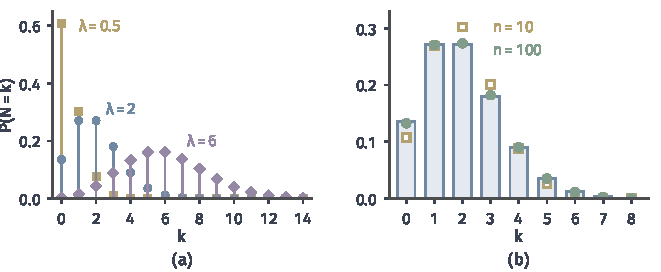
\includegraphics[width=112mm]{figures/07-probability/01-elementary-probability/matplotlib/cdist-poisson-limit/figure.pdf}
  \caption{Poisson分布。(a)$\lambda=0.5$（黄）、$2$（蓝）、$6$（紫）的质量函数。(b)浅蓝柱为$\operatorname{Poisson}(2)$，黄色空心方块为$\operatorname{Bin}(10,0.2)$，绿点为$\operatorname{Bin}(100,0.02)$，后者与柱顶几乎重合。}
  \label{fig:cdist-poisson-limit}
\end{BookInlineFigure}

\paragraph{适用范围}
定理~\ref{thm:cdist-binomial-poisson}说明了Poisson模型的一种来源：机会很多、每次很稀少、彼此独立。仅知道计数非负，并不足以采用Poisson分布。若划痕成簇出现，一道划痕附近往往还有别的，计数的方差会明显大于均值；若计数有明确的上限（例如$10$个零件中的次品数），二项分布更合适。

$\lambda=0$可以作为退化的延伸：按$0^{0}=1$的约定，式~\eqref{eq:cdist-poisson-pmf}给出$\mathbb{P}(N=0)=1$，计数恒为零。这里只把一个固定范围内的计数当作单个随机变量处理；不同时段的计数怎样联合变化、事件何时发生，属于随机过程的问题，不在本章讨论。
